\documentclass{mcmthesis}
\mcmsetup{CTeX = FALSE,   % 使用 CTeX 套装时,设置为 true
        tcn = 1900000, problem = A,
        sheet = true, titleinsheet = true, keywordsinsheet = true,
        titlepage = false, abstract = true}
\usepackage{palatino}
\usepackage{lipsum}

\usepackage{geometry}
%===============设置正文和数学字体=============================
%有些字体需要安装一些字体文件,注意辨别。
%我参照 MCM论文集的字体 使用如下宏包来定制字体。

\usepackage{graphicx}
\usepackage{subfigure}
%设置段落之间的距离,若不需要删除或者注释掉即可。
\setlength\parskip{.5\baselineskip}
\newtheorem{definition}{Definition}[section]
%\def\abstractname{Summary}%可修改摘要名称

\usepackage{indentfirst}
\setlength{\parindent}{2em}

\usepackage{chngpage}
\usepackage{array}
\usepackage{booktabs}
\usepackage{threeparttable}
\usepackage{longtable}
\usepackage[numbers,sort&compress]{natbib}
%%% 实现参考文献标号在右上角
\newcommand{\upcite}[1]{\textsuperscript{\textsuperscript{\cite{#1}}}}
%然后引用的时候使用\upcite{}的格式(一般的正常引用格式为\cite{})

\usepackage{titletoc}
\titlecontents{section}[3cm]{\bf \large}{\contentslabel{2.8em}}{}{%
\titlerule*[0.5pc]{$\cdot$}\contentspage}%
\titlecontents{subsection}[4cm]{\normalsize}{\contentslabel{2.5em}}{}{%
\titlerule*[0.5pc]{$\cdot$}\contentspage}%
\titlecontents{subsubsection}[5.3cm]{\normalsize}{\contentslabel{3.0em}}{}{%
\titlerule*[0.5pc]{$\cdot$}\contentspage}%

\title{\large The Comprehensive Evacuation Planing Model in Case of Emergency}
\author{ }


\date{\today}

\geometry{left=3.0cm,right=3.0cm}

\begin{document}


\begin{abstract}



\begin{keywords}
VRP; optimal path; Tyson polygon; Time-varying curve; \\ \hspace*{1.2cm}Time-varying curve
\end{keywords}
\end{abstract}
\maketitle
%\pagestyle{empty}
\newpage                                                          %
%==================================================================
%====================生=成=目=录===================================
\begin{adjustwidth}{-1cm}{0cm}

\setcounter{tocdepth}{3}
\thispagestyle{empty}
\tableofcontents                                                  %

\end{adjustwidth}


\newpage

\pagestyle{fancy}

\setcounter{page}{1}
\section{Introduction}
\subsection{Background}
Changes in global ocean temperature will cause various marine lives to migrate. When the temperature varies too great, these animals can no longer survive and they will migrate to more suitable habitats.

herring and mackerel are very important pelagic fish in the Scottish fisheries. herring is widely distributed throughout the Northeast Atlantic, while mackerel  is mostly distributed in the North and West Seas. They are located in the deep water during the day and move towards the surface at dusk and spread over a wide area.

It has been suggested that observed spatial variation in mackerel fisheries, extending over several hundreds of kilometers, is reflective of climate-driven changes in mackerel migration patterns. 

In recent years, with the global ocean temperature rising,  the distribution of these populations has changed dramatically. However, the geographic population shift may seriously affect the disrupt the livelihood of the smaller Scottish Fisheries companies who depend on these ocean-dwelling species.

\begin{figure}[tbp]
  \centering{
  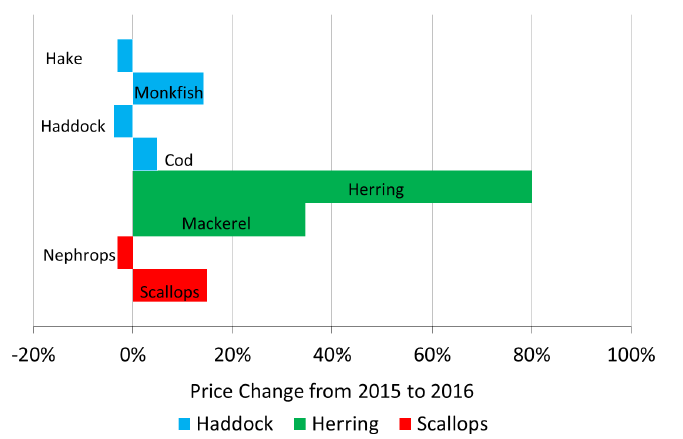
\includegraphics[width=1\textwidth]{./picture/figure3.png}}
  \caption{ Percentage change from 2015 to 2016 in the real term price per tonne obtained for key fish species}\label{figure3}
\end{figure}

\subsection{Problem Restatement}
In order to develop the Scottish fishing industries steadily,   we need to analyze the characteristics, requirements, and interactions of herring and mackerel

1.    How does the location of herring and mackerel change according to temperature

2.    What are the best case, worse case and most likely time about  small fishing companies  based on the rate 


3.    Whether these small fishing companies should change the way they operate, what is the best way to run a small fishing company
 
4.    What will happen if a certain percentage of fishery enters the territorial seas of another country

5.    What solutions will improve the future business prospects of fishermen



\subsection{Our Work}


\section{Assumptions}

\begin{itemize}
\item 
\item 
\end{itemize}

\section{List of Notation}

\begin{center}
\begin{longtable}{p{.1\textwidth}p{.8\textwidth}m{.4\textwidth}}
\caption{The List of Notation}\\
\hline
Symbol& Meaning \\
\hline

$L$      & The length of the Scottish vessels
                                                         \\
$B$      & The width of the Scottish vessels 
                                                          \\
$D$     & The height of the Scottish vessels 
                                                        \\
$W$     & The weight of the Scottish vessels 
                                                        \\
 $P$      & The   waterline length of the Scottish vessels
                                                        \\
$l$       & Length between perpendiculars                                                           \\
$v$      & The average velocity  of the Scottish vessels                                            \\
$P$      & The average power of the Scottish vessels
                                                        \\
$V$      & The displacement of the Scottish vessels 
                                                          \\
$V_o$      & The volume of the fuel consumption
                                                          \\
$A_1$     & Total purchase cost of a Scottish vessel
                                                        \\
$A_2$       & Total salary of a crew member                                                           \\
$A_3$      & Total fuel cost of a Scottish vessel                                        \\
$A$      & total cost of a Scottish vessel                                        \\
$c_1$     & The purchase cost of a Scottish vessel per hour
                                                        \\
$c_2$       & The salary of a crew member per hour                                                     \\
$c_3$      & The fuel cost of a Scottish vessel per hour                                       \\

$T_1$     & The time spent in fishing of a Scottish vessel   
                                                        \\
$T_2$       & Fish preservation time at ambient temperature        \\
$T_3$      & The time spent in sailing of a Scottish vessel     \\
$S$      & The distance sailed of a Scottish vessel   \\
$a$      & Fish density ratio \\
$r_o$      & Fuel consumption ratio \\
$B_1$      & The earnings  of herrings \\
$B_2$      & The earnings  of mackerels  \\
$p_1$      & The price  of herrings \\
$p_2$      & The price  of mackerels  \\






 \end{longtable}
 \end{center}

 \section{The fish accumutation model}
 \subsection{The varying temperature model}
 \cite{long2014fast}
 \subsubsection{basic idea}
    There are many factors can affect the temperature of the oscan, and the changing of the sea surface temperature(SST) can be 
    regarded as short monthly average temperature change and long-term yearly average temperature change from a time perspective, and spatial distribution from geographical perspective. We separate those changing trend by analyzing the data from project ERSST which contains 1$\deg$ resolution data from 1981 to 2010 and 2$\deg$ data from 1854 to 2020. Specificly, we use the long-term data to predicte the yearly change, and use high resolution data to be the begining of long-term prediction as well as to analyze the spatial distribution and the monthly change. The area we analyze lies in W15.5 to E13.5 and N46.5 to 65.5.
  \subsubsection{monthly changing}
    In our model, we assume that the monthly change has a central value related to yearly avarage temperature. We also assume that the monthly change are determined by the seasonal change and not only independent of the factors affect the change of yrarly avachange temperature, but also much stronger than the change of yearly average temperature. 
    A long-term monthly avarage are made based on SST data from 1981 to 2010. Since the seasonal change of temperature are mostly related to the rotation of the earth, it is convenience to suppose this change has a trigonometric form. 

 \subsection{The fish-temperature model}
  As we known, fish need the proper habitat to service, and temperature play an important role in multiply of fish, such as the mackerel population is found further upstream in warmer waters as the current cools through winter\cite{jansen2012migration}. In our previous predictions, the increase of  SST because global warming is obvious, so we take fisheries data  from The International Council for the Exploration of the Sea(ICES) and make a comparison. 

  \begin{figure}[tbp]
    \centering{
    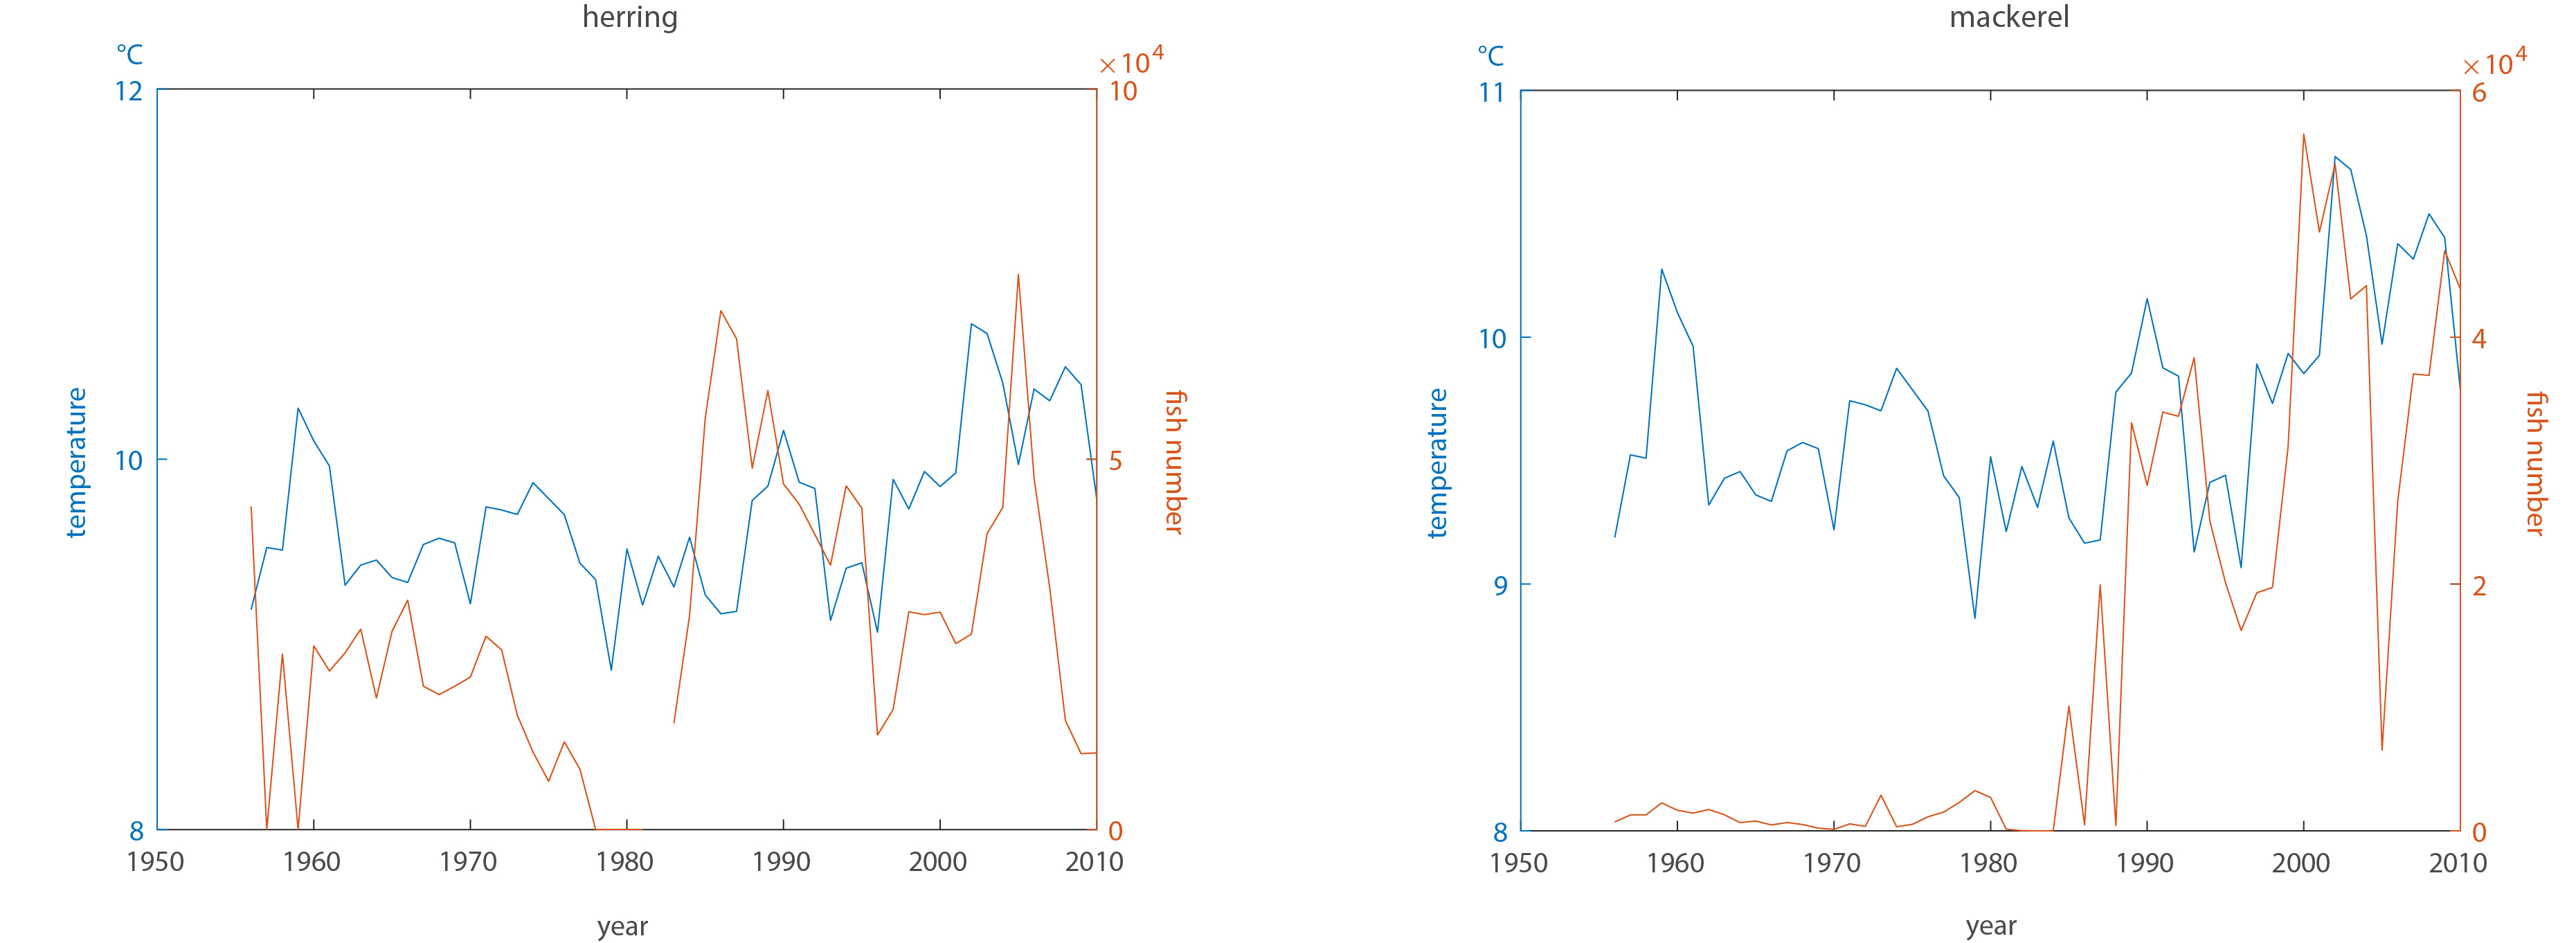
\includegraphics[width = .8\textwidth]{./fish-temp.jpg}}
    \caption{Comparison graph}\label{figure1}
  \end{figure}

  According to the graph, we can tell that besides fisheries productivity growth and some statistical gaps, the density of fish is particularly relevant to SST. So we use Pearson correlation coefficient to correlation analysis. 

  \begin{table}[!htb]
    \centering
    \setlength{\abovecaptionskip}{0pt}%
    \setlength{\belowcaptionskip}{15pt}%
    \caption{The result of correlation analysis}
    \begin{tabular}{ccccccccc}
    \toprule[1.5pt]
    result &herring &mackerel\\
    \toprule[1.5pt]
    r&0.4637&0.5463\\
    \bottomrule[1.5pt]
    \end{tabular}
  \end{table}

  So it's highly correlative. Then we use them to fitting the Gaussian distribution, and get the desired relationship between temperature and fish density.

  \begin{figure}[tbp]
    \centering{
    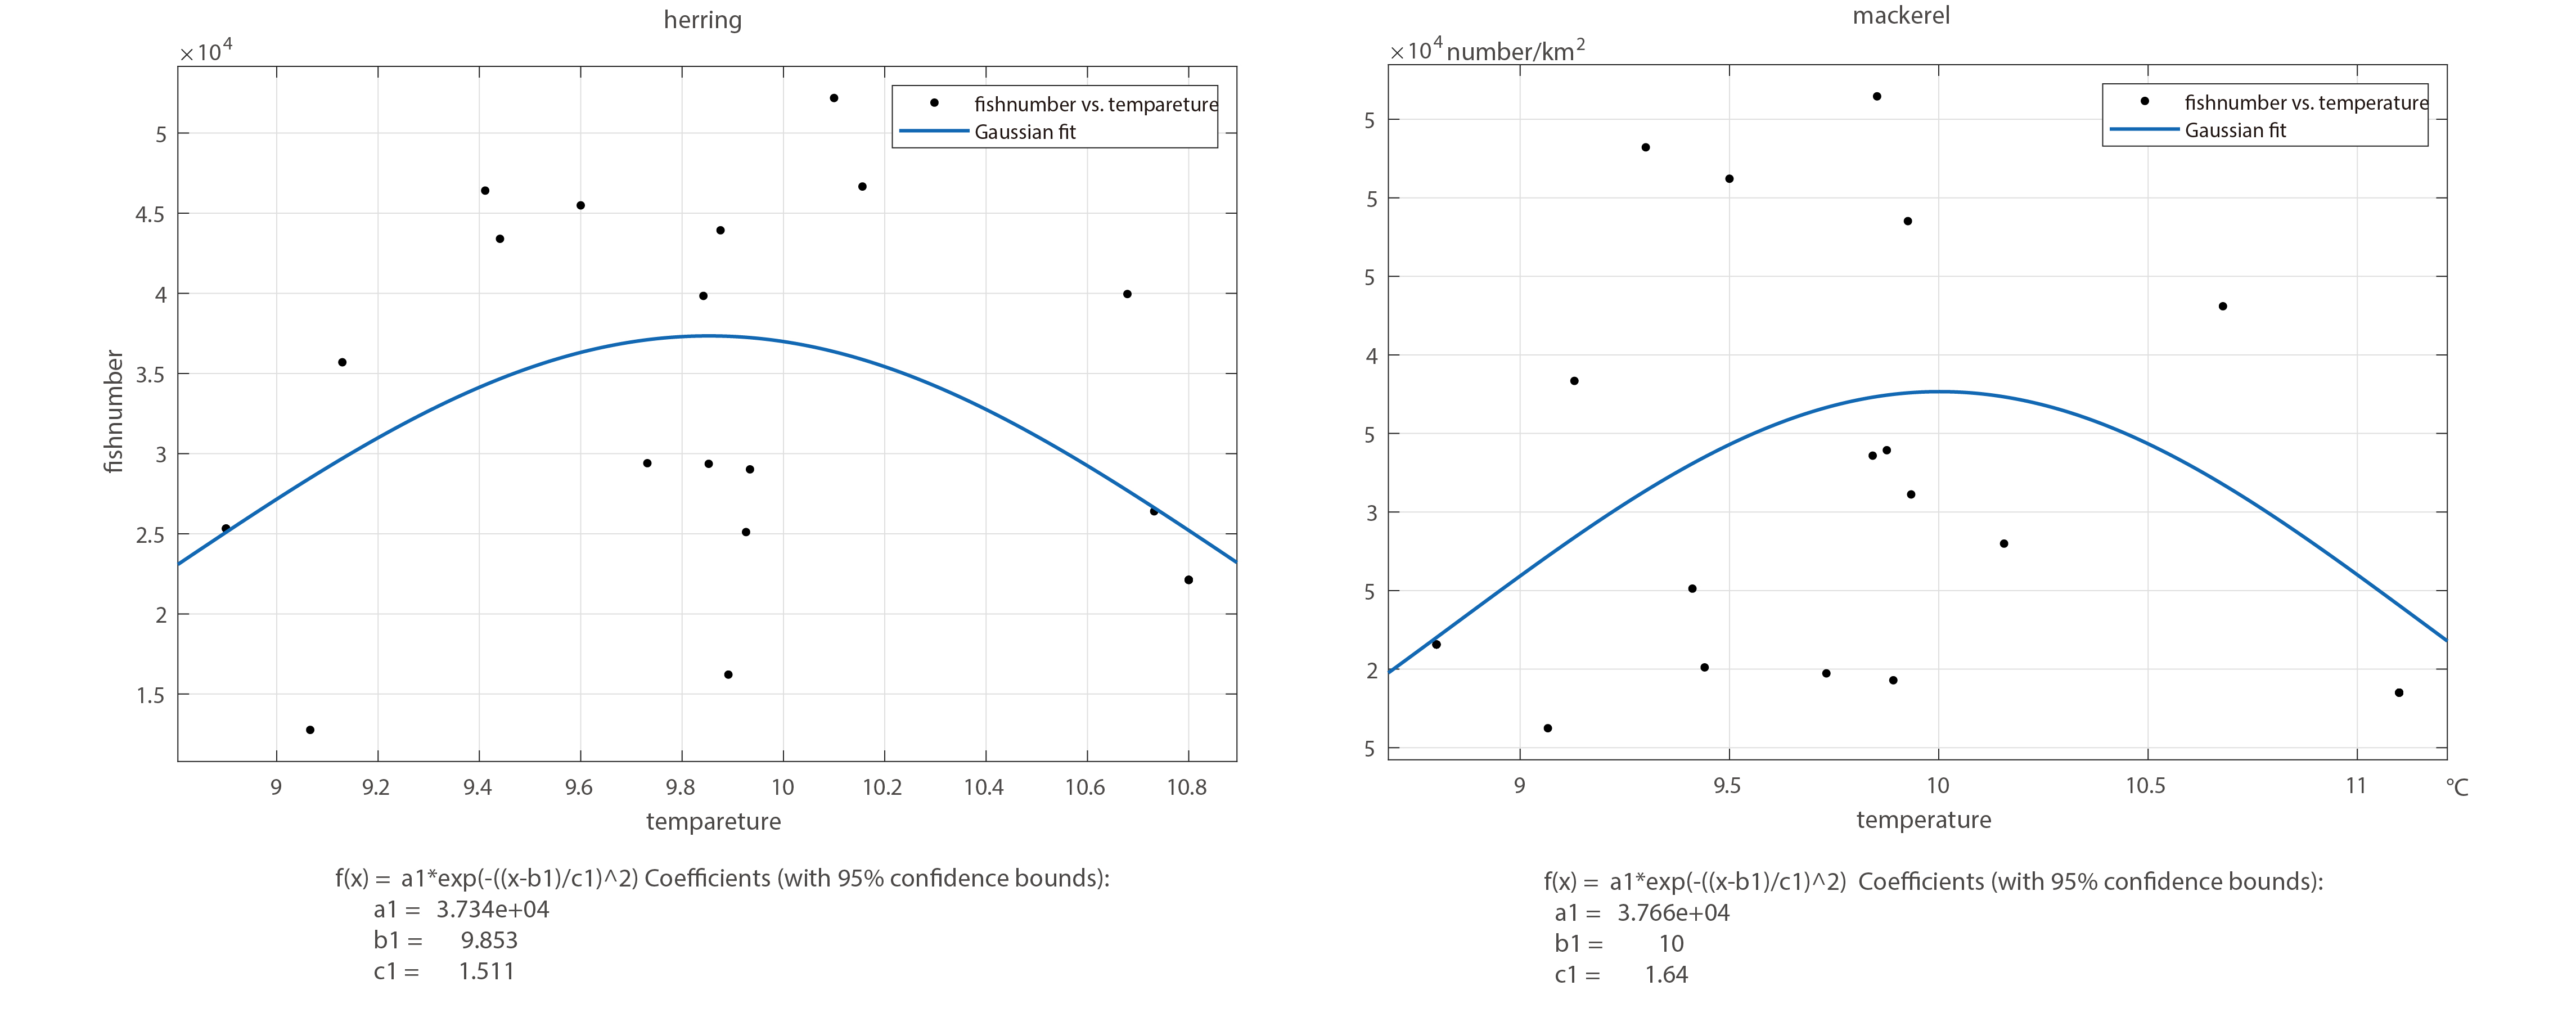
\includegraphics[width = .8\textwidth]{./fish-temp_fitting.jpg}}
    \caption{Fitting result}\label{figure1}
  \end{figure}

  \subsection{The predicted fish accumutation distribution}


\section{The Demand Distribution Model}
\begin{figure}[tbp]
  \centering{
  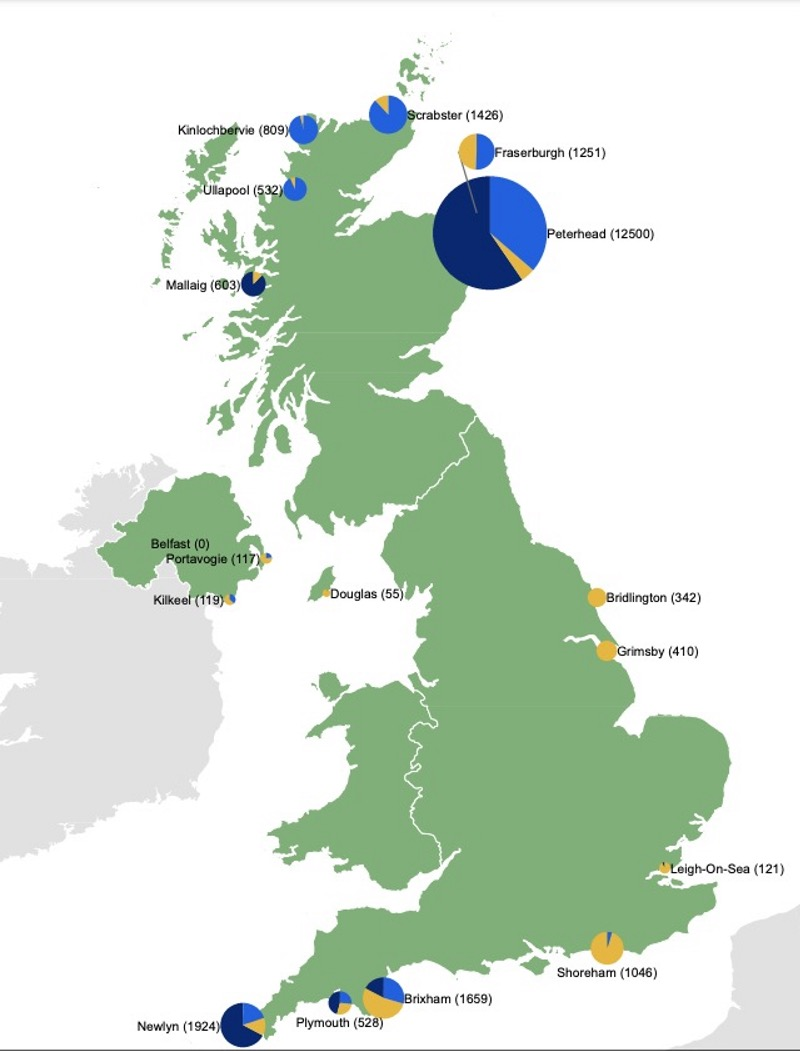
\includegraphics[width=0.6\textwidth]{./picture/figure1.jpeg}}
  \caption{English Harbor Division}\label{figure1}
\end{figure}



\begin{table}[!htb]
\centering
\setlength{\abovecaptionskip}{0pt}%    
\setlength{\belowcaptionskip}{15pt}%
\caption{The range dimension ratios of  trawlers}
\begin{tabular}{ccccccccc}
\toprule[1.5pt]
parameter &L/B&B/d&D/d\\
\toprule[1.5pt]
Range of steel materials&3.93-5.00&2.38-3.65&1.19-1.38\\
Range of wood materials&3.19-4.53&2.61-4.67&1.06-1.44\\
\bottomrule[1.5pt]
\end{tabular}
\end{table}

\begin{table}[!htb]
\centering
\setlength{\abovecaptionskip}{0pt}%    
\setlength{\belowcaptionskip}{13pt}%
\caption{The prices (pround  per tonne) of two species : 2012 to 2016}
\begin{tabular}{ccccccc}
\toprule[1.5pt]
Year&2012&2013&2014&2015&2016&average\\
\bottomrule[1.5pt]
Herring &565&408&308&369&665&463\\
Mackerel &1034&979&832&664&895&880.8\\
\bottomrule[1.5pt]
\end{tabular}
\end{table}


\begin{table}[!htb]
\centering
\setlength{\abovecaptionskip}{0pt}%    
\setlength{\belowcaptionskip}{13pt}%
\caption{The information about Scottish registered vessels}
\begin{tabular}{ccccccc}
\toprule[1.5pt]
vessel length (metres)&<=10&10-12&12-15&15-24&24-40&>=40\\
\bottomrule[1.5pt]
Herring (tonnes)&0&0&0&7&1505&63031\\
Mackerel (tonnes) &811&0&0&42&3802&183831\\
Average tonnage of &4&13&22&110&273&1748\\
Average age&26&33&29&31&28&17\\
Average engine power (kW)&57&127&190&325&641&4327\\

\bottomrule[1.5pt]
\end{tabular}
\end{table}

\begin{equation}
\left\{
\begin{array}{lr}
v=1.84\times \ (\frac{P}{V}) ^{0.237} \times \sqrt{l} &\\
l=L\approx 40 &\\
P=4000&\\
V=L\times B\times\ d =\frac{1}{48\times L^3}\\
\end{array}
\right.
\end{equation}

\begin{equation}\label{5}
T=\frac{S}{v}
\end{equation}

\begin{equation}\label{5}
A_1=c_1 \times T_1
\end{equation}

\begin{equation}\label{6}
A_2=c_2  \times T_1
\end{equation}

\begin{equation}\label{7}
A_3=c_3  \times T_1
\end{equation}

\begin{equation}\label{8}
A=A_1+A_2+A_3
\end{equation}
Where:

$C(t)$ is the cumulative percentage of withdrawal demands from time to time;

$a$ is the loading rate or the reaction rate of the public to the evacuation instructions, also expressed as the slope of the time curve;

$h$ is the time required for half of the demand in the system;

$t$=0 represents the time the evacuation order is released.



\begin{equation}\label{9}
B=1800 \times 10\% \times a \times \frac{p_1+p_2}{2}
\end{equation}


\begin{equation}\label{10}
\frac{T_1}{2}\leq T_2
\end{equation}

\begin{figure}[tbp]
  \centering{
  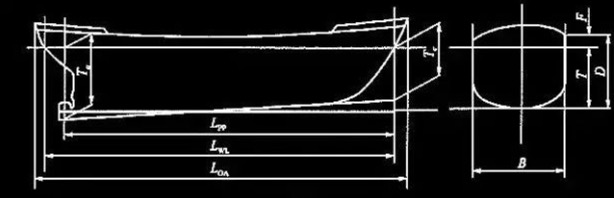
\includegraphics[width=1\textwidth]{./picture/figure2.jpeg}}
  \caption{The model of a ship}\label{figure1}
\end{figure}
 

\begin{itemize}

\item Those who have been registered to evacuate will change their minds and evacuate by private cars or other means, reducing the need for evacuation;
\item Personnel who have not been registered prepare to evacuate, including tourists or travel agents, and increase evacuation demand.

\end{itemize}





\begin{equation}\label{1}
C(t) = \frac{1}{{(1 + {e^{ - \alpha (t - h)}})}}
\end{equation}

\begin{equation}\label{2}
C(0) = 0
\end{equation}



time is crucial~\cite{Sayyady2010Optimizing,So2010Managing}.



as is shown in Figure ~\ref{figure1}.



\section{The Comprehensive Evacuation Planning Model}

\begin{equation}\label{1}
v=1.84\times \ (\frac{P}{V}) ^{0.237} \times \sqrt{l}
\end{equation}

\begin{equation}
\left\{
\begin{array}{lr}
P_0=P \times (1-0.2) &\\
P_0=(25.278\times L -169.31)
\end{array}
\right.
\end{equation}



\begin{equation}\label{3}
V=L\times B\times\ d =\frac{1}{48\times L^3}
\end{equation}

\begin{equation}\label{4}
l=L\approx 40
\end{equation}

\begin{equation}\label{4}
T_1=\frac{S}{v}
\end{equation}


			\begin{equation}
			\left\{
			\begin{array}{lr}

A_1=k_1 \times T_1\times L  &\\
A_2=c_4  \times T_1  &\\
A_3=c_3  \times T_1 &\\
A=A_1+A_2+A_3 \\		
			\end{array}
			\right.
			\end{equation}



\begin{equation}
\left\{
\begin{array}{lr}
B_0=B \times 10\% \times a \times \frac{p_1+p_2}{2} &\\
B=(12.441\times L -130.82)
\end{array}
\right.
\end{equation}


\begin{equation}\label{10}
\frac{T_1}{2}\leq T_2
\end{equation}

			

\section{The Comprehensive Evacuation Planning Model}
\subsection{Model Preparation}
\begin{table}[!ht]
\caption{The categories of hurricanes}
 \renewcommand\arraystretch{1.5}
 \setlength{\abovecaptionskip}{0pt}%    
\setlength{\belowcaptionskip}{10pt}%
\begin{center}
\begin{tabular}{p{.2\textwidth}p{.2\textwidth}m{.5\textwidth}}
\toprule[1.5pt]
Category& Maximum sustained winds & Potential damage \\
 \midrule

  Category 5 & $ \geq $ 250 km/h &   Most of the buildings and detached houses were completely destroyed, and some houses were blown away completely. \\  \bottomrule[1.5pt]
 \end{tabular}
 \end{center} 
 \end{table}
\begin{itemize}

\item 
\item 
\item \end{itemize}

VRP \cite{Dikas2016Solving,He2015Model} generally defined as: on a range of clients point (location known or can be estimated) in satisfying certain constraints (such as the demand for goods, the delivery time of delivery, the vehicle capacity constraints, etc.), reasonably arrange the vehicle distribution route, making the vehicle through them in an orderly way to achieve a certain goal (such as the shortest mileage and least cost, least time, use as little as possible and so on). The representation of VPR can be seen in Figure 3.


Based on the traditional VRP, a comprehensive evacuation planning model is established to satisfy the constraint conditions:
\begin{itemize}
  \item Time constraint: the total withdrawal time is the shortest in the case of meeting all the evacuees' needs and not violating the constraints;
  \item Risk constraint: minimum risk of meeting the minimum evacuation time;
  \item Carrying capacity constraint: the number of customers on each vehicle path is limited no more than a constant;
  \item Road afford ability constraint: the total carrying capacity on the road is not allowed to exceed the road capacity;
  \item Shelter capacity constraint: the total population in the shelter shall is not allowed to exceed the capacity limit;
  \item Priority relationship constraints: the more endangered areas have priority access;
  \item Path first constraint: after every vehicle completes its mission, records its shelter and the time to reach the sanctuary, preparing for the assignment of the next mission.
\end{itemize}

Before each task, we need to update the network node demand, shelter of residual capacity and the starting position of the vehicles, where each task should be according to the last mission at the end of the vehicle at the beginning of status to the caller, get the transport vehicles in the task.

\subsection{Modeling}

We now describe an optimization model that includes the assumptions of the previous section %%\cite{Goerigk2014Combining}.

The considered time horizon is denoted by $T$. This is not the evacuation time we are aiming for, but an upper bound on the evacuation time that is needed by our model. This quantity is used to build the time expanded network.

For public transportation we assume that there is already an established set of collection points, where evacuees gather for further transportation to shelters. For each collection point it is known how many people will appear at this point in each time step. We also given a set of possible shelter location. For each such location we are given the number of people ${W_j}$ that this shelter can hold and additionally the parking space ${C_j}$ available near this shelter.

The set of buses available for the public evacuation transit is denoted by B. For simplicity, we assume that all buses have the same capacity ${N_0}$ (however, different capacities can easily be included in our model). Besides all cars carry the same number of people.

Once the used shelter locations have been chosen, the public and private traffic will pour into the shelter. The private traffic is modeled as a dynamic network flow, the public traffic (the buses) as a dynamic multi commodity network flow. The private traffic is a single commodity whereas each bus is a commodity of its own. The flow of the buses has to be chosen such that all people that need public transportation can be brought to shelter locations while respecting the bus capacity. Both flows are chosen simultaneously in a system optimal way.

The total risk exposure is given by the sum of the risks of the individual arcs over all time steps. The risk of a single arc at a time step is given by the risk value of the arc multiplied with the number of people on this arc at this time step.

Formulating these aspects mathematically, we propose the following multi-criteria mixed-integer programming model, which we call the Comprehensive Evacuation Problem (CEP)\cite{Murray2013Evacuation,Ng2015Sharp,Ng2010Reliable}

In this mixed integer program we use the following variables: $\delta _{ij}$ denotes traversal of arc (i,j) $ \in $ A. $x_{ij}^t$ denotes the spend time passing arc (i,j). $r_{ij}^t$ denotes the risk factor passing arc (i,j) at time $t$. $f_{ij}^t$ denotes the number of evacuees using cars passing arc (i,j) at time $t$. In contrast, $g_{ij}^t$ denotes the number of evacuees using bus $b$ to go from node $i$ to node $j$ at time $t$. $\eta $ represents the jam factor, which depends on the magnitude of the hurricane, the location of the landing, and the average number of evacuees passing arc (i,j) at time $t$. $B_{ij}^t$ denotes the number of bus driving on arc (i,j) at time $t$.In the same way, $C_{ij}^t$ denotes the number of car driving on arc (i,j) at time $t$. $P_j^t$  denotes the number of people in the $j$ shelter at time $t$. $r$ denotes the capacity factor.


\begin{equation}\label{3}
\Delta \min (\Delta ,R)
\end{equation}

\begin{equation}\label{4}
\Delta  \ge (2n - 1) \times \max (\sum\limits_{(i,j) \in A} {\sum\limits_{t \in T} {\delta _{ij}^tx_{ij}^t} } ) + \Delta t
\end{equation}

The objective (1) is to minimize the evacuation time $\Delta $ and the risk $R$ ,These objectives are computed using constraints (2)-(4). Constraints (2) ensure that $\Delta $ is the maximal evacuation time. The risk $R$ depends on the number of people passing a link. This relation is expressed in constraint (3)and(4).

\begin{equation}\label{5}
 R = \sum\limits_{(i,j) \in A} {\sum\limits_{t \in T} {r_{ij}^t} } (f_{ij}^t + \sum\limits_{(i,j) \in A} {{\rm{g}}_{ij}^t} ) + W + V
\end{equation}

\begin{equation}\label{6}
\sum\limits_{(i,j) \in A} {\sum\limits_{t \in T} {f_{ij}^t} }  = {N_i} \times a\%
\end{equation}

\begin{equation}\label{7}
n = \left[ {\frac{{{N_{\rm{i}}} \times (1 - a\% )}}{{{B_i} \times {N_0}}}} \right]{\rm{ + }}1
\end{equation}

\begin{equation}\label{8}
x_{ij}^t = \eta \frac{{{S_{ij}}}}{{{v_b}}}
\end{equation}

\begin{equation}\label{9}
{\rm{g}}_{ij}^t = {N_0} \times B_{ij}^t
\end{equation}

\begin{equation}\label{10}
C_{ij}^t{\rm{ = p}} \times {{\rm{C}}_i}
\end{equation}

In the equation (5), $n$ means the number of journeys that the bus needs to transport, and the calculation should Integer plus one. Equation (8) - (10) is the road traffic that is used to constrain not to exceed its maximum capacity at time $t$.

\begin{equation}\label{11}
B_{ij}^t = {\rm{p}} \times {{\rm{B}}_i}
\end{equation}

\begin{equation}\label{12}
C_{ij}^t + B_{ij}^t \le {V_{ij}}
\end{equation}

The individual and the public traffic are linked together in the edge capacity constraints (11)-(12). Each used shelter must supply enough parking space and enough room to support evacuees.

\begin{equation}\label{13}
C_j^t \le {C_j}
\end{equation}

\begin{equation}\label{14}
P_j^t \le r{W_j}
\end{equation}

\begin{equation}\label{15}
r = \frac{{{N_{\rm{i}}}}}{{{W_j}}}
\end{equation}

When a hurricane is stronger, it may require a massive evacuation, that is, to consider the interaction of the three states. The site selection, risk coefficient, road congestion, and site accommodation will be affected, we need to reset the influence parameters to get the minimum required time and the site situation again.

Optimization method: When the forecast hat hurricane level is high, we can arrange inland evacuation ahead, in the case of ensure the overall time is enough for the coastal areas to evacuate to the site of the corresponding time calculation.

Advantage: Inland remove first can reduce the road pressure; Coastal remove later can increase the economic benefit.Compare the results again and get the final optimization plan.

\subsection{Model Solution}
Based on the above model and the parameters involved in the model, the final evacuation time is obtained by programming, and the result is shown in the table below:
\begin{table}[!htb]
\centering
\setlength{\abovecaptionskip}{0pt}%    
\setlength{\belowcaptionskip}{10pt}%
\caption{The Evacuation time}
\begin{tabular}{ccccccc}
\toprule[1.5pt]
Hurricane level &1&2&3&4&5&6\\
Evacuation time &11.4&18.2&24.28&33.6&47.8&49.6\\
\bottomrule[1.5pt]
\end{tabular}
\end{table}
%\begin{figure}[h]
%  \centering{
%  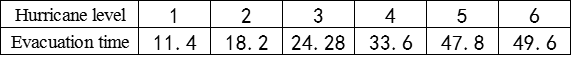
\includegraphics[width=0.7\textwidth]{./picture/figure4.png}}
%  \caption{The Evacuation Time}\label{Table1}
%\end{figure}



As shown in the figure above, it is necessary to calculate the time required for a category 1- 5 hurricane, including the withdrawal time required for the optimization programme.

Because the evacuation and time of personnel also satisfied the curve of $S$ type curve, it can be used to draw the time-varying personnel evacuation curve of hurricane from category 1 - 5, which can be seen in figure4.



On the basis of guarantee the safety of life, we put forward the optimization scheme, when hurricane prediction level too high, let let evacuated inland areas, in order to improve the economic benefit of coastal, and reduce economic loss. The maximum population density due to coastal areas, and abide by the $S$ type curve evacuation rules.


Under the same Five - level hurricane conditions, the optimization scheme minimizes the economic loss under the conditions of increasing the cost of the smaller time. It has been proved that evacuating in the right time can get better effect, which has a positive effect on the subsequent development of evacuation plan.

\section{Strengths and Weaknesses}

\subsection{Strengths}

\begin{itemize}
  \item The comprehensive evacuation planning model takes the shortest time and lowest risk and low economic losses as the total constraint conditions to get the optimal solution;
  \item The constraint conditions such as road carrying capacity and the capacity of escape points are considered in the comprehensive evacuation planning model;
  \item Determine the coverage scope by Thiessen polygon;
  \item Considering the demand distribution characteristics in the station nodes;
  \item In terms of model constraints, the shortest evacuation time is obtained for a 1-5 hurricane;
  \item Considering the economic benefit gap between inland and coastal areas, the optimal plan for economic loss is proposed;
  \item Analyze the extreme problems, propose solutions, and obtain the optimal solution through comprehensive consideration of evacuation time, evacuation risks and economic losses.
\end{itemize}

\subsection{Weaknesses and Extensions}
\begin{itemize}
  \item Without considering the evacuation of the county itself;
  \item Without considering the refueling problem of cars and buses;
  \item Without considering the risk caused by large numbers of people in station nodes;
  \item Without considering other means of transportation, such as aircraft, railway, etc.;
  \item Without considering the subsequent material problems of the shelter.
\end{itemize}

Optimization method: When the forecast hat hurricane level is high, we can arrange inland evacuation ahead, in the case of ensure the overall time is enough for the coastal areas to evacuate to the site of the corresponding time calculation.

Advantage: Inland remove first can reduce the road pressure; Coastal remove later can increase the economic benefit. Compare the results again and get the final optimization plan.

\addcontentsline{toc}{section}{Reference}
\bibliographystyle{plain}
\bibliography{myreference}

\begin{appendices}

\section{First appendix}

\lipsum[13]

Here are simulation programmes we used in our model as follow.\\

\textbf{\textcolor[rgb]{0.98,0.00,0.00}{Input matlab source:}}
% \lstinputlisting[language=Matlab]{./code/mcmthesis-matlab1.m}

\section{Second appendix}

some more text \textcolor[rgb]{0.98,0.00,0.00}{\textbf{Input C++ source:}}
% \lstinputlisting[language=C++]{./code/mcmthesis-sudoku.cpp}

\end{appendices}
\end{document}
